\documentclass[a4paper,10pt]{article}
\usepackage[margin=1in]{geometry}
\usepackage{amsmath,amsthm,amssymb,amsfonts,stmaryrd}
\usepackage{soul}
\usepackage{array}
\usepackage{empheq}
\usepackage{xfrac}
\usepackage{minibox}
\usepackage{enumitem}
	\setlist{nosep} % or \setlist{noitemsep} to leave space around whole list
\usepackage{color}
\usepackage{blkarray}
\setcounter{MaxMatrixCols}{20}
\usepackage{showlabels}
\usepackage{arydshln}	% Dotted lines in arrays
\usepackage{adjustbox}
\usepackage{hyperref}
\hypersetup{
  colorlinks   = true, %Colours links instead of ugly boxes
  urlcolor     = blue, %Colour for external hyperlinks
  linkcolor    = blue, %Colour of internal links
  citecolor   = red %Colour of citations
}
\usepackage{cleveref}


\newtheorem{lemma}{Lemma}
\newtheorem{definition}{Definition}
\newtheorem{theorem}{Theorem}
\newtheorem{corollary}{Corollary}

\newcommand{\tcb}{\textcolor{blue}}
\newcommand{\todo}[1]{\textcolor{red}{[TODO\@: #1]}}


\begin{document}
\allowdisplaybreaks

% ----------------------------------------------------------------------------------------------------------- %
% ----------------------------------------------------------------------------------------------------------- %
% ----------------------------------------------------------------------------------------------------------- %
\section{Introduction}

% ----------------------------------------------------------------------------------------------------------- %
% ----------------------------------------------------------------------------------------------------------- %
\subsection{Fully implicit Runge-Kutta}

Consider the method-of-lines approach to solving partial differential equations (PDEs),
where we discretize in space and arrive at a system of ODEs in time,
%
\begin{align}\label{eq:problem}
	M\mathbf{u}'(t) =  \mathcal{N}(\mathbf{u},t) \quad\text{in }(0,T], \quad \mathbf{u}(0) = \mathbf{u}_0,
\end{align}
%
where $M$ is a mass matrix, and $\mathcal{N}\in\mathbb{R}^{N\times N}$ a discrete, time-dependent, nonlinear
operator depending on $t$ and $\mathbf{u}$ (including potential forcing terms).
Then consider time propagation using an $s$-stage
Runge-Kutta scheme, characterized by the Butcher tableaux 
%
\begin{align*}
	\renewcommand\arraystretch{1.2}
	\begin{array}
	{c|c}
	\mathbf{c}_0 & A_0\\
	\hline
	& \mathbf{b}_0^T
	\end{array},
\end{align*}
%
with Runge-Kutta matrix $A_0 = (a_{ij})$, weight vector $\mathbf{b}_0^T = (b_1, \ldots, b_s)^T$, and 
nodes $\mathbf{c}_0 = (c_0, \ldots, c_s)$.

Runge-Kutta methods update the solution using a sum over stage vectors,
%
\begin{align*}
\mathbf{u}_{n+1} & = \mathbf{u}_n + \delta t \sum_{i=1}^s b_i\mathbf{k}_i, \\
M\mathbf{k}_i & = \mathcal{N}\left(\mathbf{u}_n + \delta t\sum_{i=1}^s b_i\mathbf{k}_i, t_n+\delta tc_i\right).
\end{align*}
%
For nonlinear PDEs, $\mathcal{N}$ is linearized using, for example, a Newton or a Picard
linearization of the underlying PDE. Let us denote this linearization $\mathcal{L}\in\mathbb{R}^{N\times N}$
(or, in the case of a linear PDE, let $\mathcal{L} := \mathcal{N}$).
Expanding, solving for the stages $\mathbf{k}$ as each step in a nonlinear iteration, or
as the update to $\mathbf{u}$ for a linear PDE, can then be expressed as a block linear system,
%
\begin{align}\label{eq:k0}
\left( \begin{bmatrix} M  & & \mathbf{0} \\ & \ddots \\ \mathbf{0} & & M\end{bmatrix}
	- \delta t \begin{bmatrix} a_{11}\mathcal{L}_1 & ... & a_{1s}\mathcal{L}_1 \\
	\vdots & \ddots & \vdots \\ a_{s1}\mathcal{L}_s & ... & a_{ss} \mathcal{L}_s \end{bmatrix} \right)
	\begin{bmatrix} \mathbf{k}_1 \\ \vdots \\ \mathbf{k}_s \end{bmatrix} 
& = \begin{bmatrix} \mathbf{f}_1 \\ \vdots \\ \mathbf{f}_s \end{bmatrix}.
\end{align}
%

The difficulty in fully implicit Runge-Kutta methods (which we will denote IRK) lies in
solving the $Ns\times Ns$ block linear system in \eqref{eq:k0}. This paper focuses on the
parallel simulation of numerical PDEs, where $N$ is typically very large, on the order of
millions or billions, and $\mathcal{L}$ is highly ill-conditioned. In such cases, direct
solution techniques to solve \eqref{eq:k0} are not a viable option, and fast, parallel 
iterative methods must be used. However, IRK methods are rarely employed in practice due
to the difficulties of solving \eqref{eq:k0}. Even for relatively simple
parabolic PDEs where $\mathcal{L}$ is symmetric positive definite, \eqref{eq:k0}
instead yields a large nonsymmetric system with significant block coupling. For
nonsymmetric systems $\mathcal{L}$ that already have variable coupling, fast iterative
methods are even less likely to yield acceptable performance in solving \eqref{eq:k0}.

A standard approach for IRK methods is to assume $\mathcal{L}_i = \mathcal{L}_j$ for all $i,j$,
that is, $\mathcal{L}$ has no dependence on time. For nonlinear problems, this correspond to
a simplified Newton method, where the Jacobian is only evaluated at one time-point per time
step (or also naturally arises for a linear problem with no time-dependence in spatial
differential components). This yields a simplified form of \eqref{eq:k0} that can be
expressed in Kronecker product form,
%
\begin{align}\label{eq:kron1}
(I\otimes M - \delta t A_0\otimes \mathcal{L})\mathbf{k} & = \mathbf{f},
\end{align}
%
where $\mathcal{L}$ is a real-valued spatial operator or Jacobian independent of time.
Here, we build on some of the older Runge-Kutta work in the light of a changing
computational landscape, developing a new iterative approach to solve \eqref{eq:kron1}.
The new method effectively requires $s$ real-valued linear solves of matrices along the
lines of $M - \delta t\eta\mathcal{L}$, for some $\eta > 0$. 



% ----------------------------------------------------------------------------------------------------------- %
% ----------------------------------------------------------------------------------------------------------- %
\subsection{The time-independent case}

The Kronecker product form (resulting from the assumption that $\mathcal{L}$ is independent of
time) allows for further simplifications. First proposed in \todo{Butcher77}, let $A_0$ have
Jordan normal form $A_0 = U_0L_0U_0^{-1}$, where $L_0$ is lower triangular, with eigenvalues
of $A_0$ on the diagonal and lower triangular entries corresponding to the (unit-valued)
Jordan blocks. Then \eqref{eq:kron1} is equivalent to the problem
%
\begin{align}\label{eq:kron2}
(U_0\otimes I)(I\otimes M - \delta t L_0\otimes \mathcal{L})(U_0^{-1}\otimes I)\mathbf{k} & = \mathbf{f},\\
(I\otimes M - \delta t L_0\otimes \mathcal{L})\hat{\mathbf{k}} & = \hat{\mathbf{f}},
\end{align}
%
where $\hat{\mathbf{f}} := (U_0^{-1}\otimes I)\mathbf{f}$ and
$\hat{\mathbf{k}} := (U_0^{-1}\otimes I)\mathbf{k}$. Note that computing the Jordan
decomposition of $A_0$ is typically of trivial computational expense compared to other
operations. The transformed system in \eqref{eq:kron2} can now be inverted by applying
a block diagonal or lower triangular solve, which only requires inverting the diagonal
blocks, $M - \delta_t(L_0)_{ii}\mathcal{L}$.

Transforming \eqref{eq:kron1} into \eqref{eq:kron2} reduces the solution of an $ns\times ns$
system of equations to solving $s$ linear systems of size $n\times n$. The downside is that the
IRK schemes with high accuracy and stability have primarily complex eigenvalues, in which case
the original real-valued system was transformed into a set of smaller complex systems (if the
original matrix $\mathcal{L}$ is complex, obviously complex eigenvalues are not a concern).
Complex eigenvalues introduce several difficulties. First, complex operations require several
times the floating-point operations to perform standard algebraic operations. Second, not
all preconditioners are well-developed for complex-valued matrices. Last, an important
practical concern is that not all software libraries support complex numbers. 

Published shortly after (and independently from) Butcher's result regarding Jordan normal
form \todo{cite}, Bickart developed a similar result \todo{cite}. If we define $Q_s(x)$ as the characteristic
polynomial of $A_0$, then the inverse of \eqref{eq:kron1} can be computed via some matrix-vector
multiplications and the action of $Q_s(\mathcal{L})^{-1}$ \todo{cite}. This is similar in principle to
Butcher's result, as in practice one could invert $Q_s(\mathcal{L})$ by inverting 
each term in the factored polynomial, $(\mu_1 I-\mathcal{L})^{-1}$,
$(\mu_2 I-\mathcal{L})^{-1}$, ..., for eigenvalues $\{\mu_i\}_{i=1}^s$ of $A_0$.
Although Bickart's paper received less attention than Butcher's over time (currently $2.5\times$
less citations), the polynomial form provides a more natural way to handle complex eigenvalues,
particularly in the modern high-performance computing landscape, where direct LU inverses
are rare and most linear systems are solved via preconditioning and/or Krylov methods. 

\todo{Fix discussion on Bickart's result, work out what he actually did carefully.}

% ----------------------------------------------------------------------------------------------------------- %
% ----------------------------------------------------------------------------------------------------------- %
\subsection{Why IRK and previous work}


 compared with simpler options such as
diagonally implicit Runge Kutta (DIRK) methods, where $A_0$ and \eqref{eq:k0} are 
(block) lower triangular; then, the solution of \eqref{eq:k0} only requires $s$ linear
solves of $M - \delta ta_{ii}\mathcal{L}_i$. 




Fully implicit Runge-Kutta (IRK) methods offer a number af advantages in terms of stability and
accuracy, particularly for difficult nonlinear PDEs. However, the solution of \eqref{eq:k0}
remains difficult and limits the use of fully implicit RK methods in numerical PDEs.
Diagonally implicit RK (DIRK) methods address this problem by constructing $A_0$ to be lower
triangular, in which case \eqref{eq:k0} is easily inverted by inverting the diagonal
blocks, $M - \delta ta_{ii}\mathcal{L}_i$ for $i=1,..,s$. However, DIRK methods attain
lower global orders of accuracy than IRK methods, and have at most stage-order one (stage-order
two with one explicit stage). This is particularly problematic in terms of order reduction,
an interesting phenomenon of using RK methods with the method-of-lines approach to solve PDEs,
where error in spatial boundary conditions for intermediate RK stages limits the achieved space-time
accuracy. The concept is not fully understood, nor are there many practical fixes for PDEs
in higher than one dimension. However, for nonlinear PDEs, it is typically the case that the global 
order of accuracy is limited to $\approx \min\{ p, q+1\}$, for integration order $p$ and stage-order
$q$. Obviously if we actually want high-order integration in time, SDIRK and ESDIRK methods
are limiting, and fully implicit high-order RK methods are desirable. Unfortunately, solving the
fully implicit stage matrix in \eqref{eq:k0} is often much more difficult when it is not lower triangular.
Here we consider new block preconditioning techniques to facilitate this.

% Simplified newton scheme uses fixed Jacobian for all stages
% Single step Newton (Cooper (83/90), Gonzales-Pinto (95/97)
% ---------------- ODEs and LU ---------------- %
Butcher (76), Bickart (77)
\begin{itemize}
	\item Uses tensor product structure, gets Jordan normal form of Butcher matrix A. Reformulates
	problem as block subdiagonal, with diagonal blocks $I - h\lambda J$, for Jacobian $J$, time step $h$,
	and eigenvalue $\lambda$ of $A$ (are we sure not $A^{-1}$??).
	\item Must solve for complex eigenvalues. This is not desirable. 
	\item Bickart uses polynomial form, closer to what I look at. Originally based on Tensor product
	result from Jameson (68)
\end{itemize}

Varah (79):
\begin{itemize}
	\item Much better description of Butcher's method. Transforms coordinate system of Jacobian tensor.
	Still relies on this tensor structure to do said transformation. 
	\item Transforms Jacobian to Hessenberg form to avoid repeated action computing LU of a shifted 
	Jacobian.
\end{itemize}

Burrage (82):
\begin{itemize}
	\item Look at stability of DIRK and SIRK methods, which have one eigenvalue and are more amenable
	to development by Butcher. 
\end{itemize}

Orel (91):
\begin{itemize}
	\item Looks at RK methods w/ real eigenvalues. Turns out best approximation to exponential is
	obtained by having all eigenvalues equal (SIRK/SDIRK methods). SIRK methods offer some advantages over SDIRK methods, but lack the favorable stabillity an accuracy of IRK methods. 
\end{itemize}

Cooper:
\begin{itemize}
	\item (83,90,93): develops single Newton scheme using SOR or various matrix splittings,
	applied to ODEs. This is a single-step
	Newton method, where the actual Jacobian solve is replaced with an SOR iteration. Here, Butcher
	matrix A is replaced with an approximate matrix with one positive real eigenvalue. 
\end{itemize}

Pinto:
\begin{itemize}
	\item (95) Mostly ODEs, do consider 1d-space-1d-time burgers on a very small grid. 
	\item (96) additional iteration of single Newton, makes it quasi-Newton like. 
	\item (01) Analysis of single Newton (SOR) w/ simplified Newton for higer order. 
\end{itemize}


Butcher (2000):
\begin{itemize}
	\item Develops ESDIRK schemes w/ higher stage order and stiff accuracy than traditional
	SIRK/DIRK schemes. Based on using iniital explicit stage, moves RK abscissae.
\end{itemize}


Brugano (2014) and Antonana (2018)
\begin{itemize}
	\item New splitting and IRK techniques for Hamiltonian problems where conservation is
	important. Used for ODEs. 
\end{itemize}


% ---------------- PDEs ---------------- %

\begin{itemize}
	\item One obvious drawback -- even if spatial operator/Jacobian is SPD, IRK system is
	nonsymmetric.
\end{itemize}

Lay (2000)
\begin{itemize}
	\item 
\end{itemize}

Van Lent (2004)
\begin{itemize}
	\item Multigrid for IRK?
\end{itemize}

Staff \& Mardal (2006)
\begin{itemize}
	\item One of first paper to consider preconditioning the fully implicit RK system.
	Use block Jacobi and block lower triangular preconditioners for the diffusion equation.
	Use multigrid V-cycles and full Newton time-dependent Jacobian. Upper triangular is
	bad compared to block Jacobi and lower triangular (this has appeared elsewhere in
	literature -- $A_0$ is dominant in lower triangular part -- Crout factorization
	in I think Messina or Van der Houwen; comes up again in Brugano (2015)).
\end{itemize}
Mardal (2007)
\begin{itemize}
	\item Analyze block-diagonal preconditioners in a Sobolev setting, demonstrate
	conditioning of the preconditioned operator to be optimal in the independent of
	$h$ sense. Use multigrid w/ diffusion as example. 
\end{itemize}
Nilssen (2011)
\begin{itemize}
	\item Analogous to above, Sobolev analysis for block-diagonal preconditioning
	applied to the bidomain equations.
\end{itemize}

Xie (2011)
\begin{itemize}
	\item Proposes a modified simplified Newton for the time-dependent cast, where the Jacobian is
	formed based on a least squares approximation to the true RK coefficients, evaluating all entries
	at a single time point. In example problems, modified Jacobian typically converged faster
	than simplified (evaluated at previous time step), up to 2x less iterations/time. 
\end{itemize}

Hao Chen:
\begin{itemize}
	\item (2014) Develops a splitting iterative method to precondition IRK matrices, similar to ADI schemes.
	Proves that for definite spatial operators and Butcher matrices (that is, eignvalues have positive
	or negative real parts), $\rho(T) < 1$, where $T$ is the fixed-point iteration matrix. Look at 
	diffusion equation with IRK and BVMs.
	\item (2016) Analogous to above, extended to wave equation.
\end{itemize}

Pazner
\begin{itemize}
	\item
\end{itemize}



% ----------------------------------------------------------------------------------------------------------- %
% ----------------------------------------------------------------------------------------------------------- %
% ----------------------------------------------------------------------------------------------------------- %
\section{Inverting the IRK system}

The RK stage system in \eqref{eq:k0} can be reformulated as \todo{cite Will}
%
\begin{align*}
\left( A_0^{-1}\otimes M - \delta t \begin{bmatrix} \mathcal{L}_1  & \\ & \ddots \\ && \mathcal{L}_s\end{bmatrix}\right)
	(A_0\otimes I)	\begin{bmatrix} \mathbf{k}_1 \\ \vdots \\ \mathbf{k}_s \end{bmatrix} 
& = \begin{bmatrix} \mathbf{f}_1 \\ \vdots \\ \mathbf{f}_s \end{bmatrix}.
\end{align*}
%
For ease of notation, let us scale both sides of the system by a block-diagonal mass matrix 
and, excusing the slight abuse of notation, let $\mathcal{L}_i \mapsto \delta t M^{-1}\mathcal{L}_i$,
$i=1,..,s$. Note the time step is now included in $\mathcal{L}_i$. Because $\mathcal{L}_i$ is
time-dependent, it is possible that $\delta t$ is also time-dependent.
Now let $\alpha_{ij}$ denote the $ij$-element of $A_0^{-1}$ (assuming $A_0$ is
invertible). Then, solving \eqref{eq:k0} can be effectively reduced to inverting the operator
%
\begin{align}\label{eq:k1}
\mathcal{M}_s := A_0^{-1}\otimes I - \begin{bmatrix} \mathcal{L}_1  & \\ & \ddots \\ && \mathcal{L}_s\end{bmatrix}
	& = 
\begin{bmatrix} \alpha_{11}I - \mathcal{L}_1 & \alpha_{12}I & ... & \alpha_{1s}I \\
	\alpha_{21}I & \alpha_{22}I - \mathcal{L}_2 & & \alpha_{2s}I \\
	\ddots & & \ddots & \vdots \\ \alpha_{s1}I & ... & \alpha_{s(s-1)}I & \alpha_{ss}I - \mathcal{L}_s \end{bmatrix}.
\end{align}
%
Note, there are a number of methods with one explicit stage preceded or followed by several
fully implicit and coupled stages. In such cases, $A_0$ is
not invertible, but the explicit stage can be eliminated from the system. The remaining operator
can then be reformulated as above, and the inverse that must be applied takes the form of
\eqref{eq:k1} but based on a principle submatrix of $A_0$.


% ----------------------------------------------------------------------------------------------------------- %
% ----------------------------------------------------------------------------------------------------------- %
\subsection{The case of commuting operators}

This section introduces a result similar to Bickart's but generalized to hold for commuting
operators. If $\mathcal{L}_i=\mathcal{L}_j$ for all $i,j$, we show that the inverse of
\eqref{eq:k1} can be expressed in terms of $P_s(\mathcal{L})^{-1}$, where $P_s(\mathcal{L})$
is the characteristic polynomial of $A_0^{-1}$.

%
\begin{lemma}
Let $\alpha_{ij}$ denote the $(i,j)$th entry of $A_0^{-1}$ and assume $\{\mathcal{L}_i\}_{i=1}^s$
are commuting operators. Define 
\begin{align}\label{eq:k1}
\mathcal{M}_s := \begin{bmatrix} \alpha_{11}I - \mathcal{L}_1 & \alpha_{12}I & ... & \alpha_{1s}I \\
	\alpha_{21}I & \alpha_{22}I - \mathcal{L}_2 & & \alpha_{2s}I \\
	\ddots & & \ddots & \vdots \\ \alpha_{s1}I & ... & \alpha_{s(s-1)}I & \alpha_{ss}I - \mathcal{L}_s \end{bmatrix},
\end{align}
as in \eqref{eq:kron1}.
Let det$(\mathcal{M}_s)$ be the determinant of $\mathcal{M}_s$ (in this case a block-diagonal
matrix) and let adj$(\mathcal{M}_s)$ be the adjugate of $\mathcal{M}_s$. Then, $\mathcal{M}_s$
is invertible if and only if $\mathcal{D}_s$ is invertible, and
\begin{align*}
\mathcal{M}_s^{-1} = \textnormal{det}({M}_s)^{-1}\textnormal{adj}(\mathcal{M}_s).
\end{align*}

Now, suppose $\mathcal{L}_i = \mathcal{L}_j$ for all $i,j$, and let $P_s(x)$ be the
characteristic polynomial of $A_0^{-1}$. Then,
\begin{align*}
\mathcal{M}_s^{-1} = \textnormal{diag}(P_s(\mathcal{L})^{-1})\textnormal{adj}(\mathcal{M}_s),
\end{align*}
where ``diag'' indicates a block diagonal matrix, with diagonal blocks given by $P_s(\mathcal{L})^{-1}$.
\end{lemma}
%
\begin{proof}
Notice in \eqref{eq:k1} that if $\mathcal{L}_i$ and $\mathcal{L}_j$ commute for all $i,j$,
then $\mathcal{M}_s$ is a matrix over the commutative ring of linear combinations
of $I$ and $\{\mathcal{L}_i\}$. Let adj$(\mathcal{M}_s)$ denote the matrix adjugate. A
classical result in matrix analysis then tells us that
%
\begin{align*} 
\textnormal{adj}(\mathcal{M}_s)\mathcal{M}_s = \mathcal{M}_s\textnormal{adj}(\mathcal{M}_s)
	= \textnormal{det}(\mathcal{M}_s)I.
\end{align*}
%
Moreover, $\mathcal{M}_s$ is invertible if and only if if the determinant of $\mathcal{M}_s$
is invertible, in which case $\mathcal{M}_s^{-1} := $ det$(\mathcal{M}_s)^{-1}$adj$(\mathcal{M}_s)$.
\todo{Need citations!}
For the case of time-independent operators ($\mathcal{L}_i=\mathcal{L}_j$), notice that
$\mathcal{M}_s$ takes the form $A_0^{-1} - \mathcal{L}I$ over the commutative ring defined
above. Analogous to a scalar matrix, the determinant of $A_0^{-1} - \mathcal{L}I$ is the
characteristic polynomial of $A_0^{-1}$ evaluated at $\mathcal{L}$.
\end{proof}
%

The adjugate simply consists of linear combinations of $I$ and $\mathcal{L}$, and an analytical
form can be derived (albeit tediously) for an arbitrary $s\times s$ matrix, where
$s\sim\mathcal{O}(1)$. Computing its action will consist of some set of vector summations
and matrix-vector multiplications.



{\color{blue}
\textbf{Algorithm:}
\begin{itemize}
	\item When we precondition each row of the block matrix with the same inverse
	polynomial, we can suck it out of the summation over stages. Then each stage is
	appropriately modified by $A_0^{-1}$ and the adjugate, the results are summed,
	and the preconditioner/inverse applied to the sum. This is important to limit
	the linear solves to $s$ solves. 
\end{itemize}
}



% ----------------------------------------------------------------------------------------------------------- %
% ----------------------------------------------------------------------------------------------------------- %
% ----------------------------------------------------------------------------------------------------------- %
\section{Inverting the characteristic polynomial}

% ----------------------------------------------------------------------------------------------------------- %
% ----------------------------------------------------------------------------------------------------------- %
\subsection{Stability and the method of lines}

{\color{blue}
\begin{itemize}

\item A necessary condition for stable time-propagation is that eigenvalues of $\mathcal{L}$
lie in the region of stability for the given RK scheme. For virtually all implicit RK schemes,
this means that eigenvalues of $\mathcal{L}$ must have negative real part, or real part
$\gg 0$. It is rare for operators representing a differential discretization to be split
with a set of negative definite eigenvalues and a set of eigenvalues with real part $\gg 0$,
so for our purposes assume $\mathcal{L}$ has eigenvalues with negative real part.

\item Just eigenvalues is not strong enough for our analysis or stability. Need to look
into literature. Would be nice if it was related to numerical range/field of values, because
that is what our analysis is based on. Ideally, something along the lines of $\mathcal{L}$ 
has a non-positive field of values for stability? 
\end{itemize}
}


% ----------------------------------------------------------------------------------------------------------- %
% ----------------------------------------------------------------------------------------------------------- %
\subsection{Grouping by conjugate pairs}

By computing the eigenvalues $\{\lambda_i\}$ of $A_0^{-1}$, we can express
$P_s(\mathcal{L})$ in a factored form, 
%
\begin{align}\label{eq:fac}
P_s(\mathcal{L}) = \prod_{i=1}^s (\lambda_i I - \mathcal{L}),
\end{align}
%
and its inverse can then be computed by successive applications of $(\lambda_iI - \mathcal{L})^{-1}$,
for $i=1,...,s$. As discussed previously, eigenvalues of $A_0$ and $A_0^{-1}$ will often be
complex, making the inverse of individual factors $(\lambda_iI - \mathcal{L})^{-1}$ more
difficult and often not practical. Because eigenvalues come in conjugate pairs, one simplification
can be achieved by noting that $(\overline{\lambda_i}I - \mathcal{L})^{-1}
= \overline{(\lambda_iI - \mathcal{L})^{-1}}$, and thus the same solver/preconditioner
could be used for conjugate pairs of eigenvalues \todo{cite}. However, this does not
solve the underlying problem of constructing complex solvers/preconditioners in
practice. 

Here, we take a different approach, combining the factors of conjugate eigenvalues
into a set of quadratic polynomials that we must precondition,
%
\begin{align}\label{eq:imag1}
((\eta + i\beta)I - \mathcal{L})((\eta - i\beta)I - \mathcal{L}) =
	(\eta^2+\beta^2)I - 2\eta \mathcal{L} + \mathcal{L}^2.
\end{align}
%
In practice, we typically do not want to directly precondition a quadratic operator
like \eqref{eq:imag1}. For example, a discretization of diffusion is typically 
conditioned like $1/h^2$ for mesh spacing $h$ (worse for high-order discretizations),
so considering $\mathcal{L}^2$ directly results in conditioning $\sim\mathcal{O}(1/h^4)$.
Moreover, many fast parallel methods such as multigrid are not well-suited for solving
a polynomial in $\mathcal{L}$. The point of \eqref{eq:imag1} is that by considering
conjugate pairs of eigenvalues, the resulting operator is real-valued. Thus, what if
we precondition \eqref{eq:imag1} with the inverse of the real-valued quadratic polynomial,
$(\eta I - \mathcal{L})(\eta I - \mathcal{L})$? Expanding, the preconditioned operator
takes the form
%
\begin{align}\nonumber
\mathcal{P}_A & := (\eta I - \mathcal{L})^{-2}\left[(\eta^2+\beta^2)I - 2\eta \mathcal{L} + \mathcal{L}^2\right] \\
&\hspace{5ex} = I + \beta^2(\eta I - \mathcal{L})^{-2}
= I + \frac{\beta^2}{\eta^2}\left(I - \tfrac{1}{\eta}\mathcal{L}\right)^{-2}.\label{eq:prec1}
\end{align}
%

We will now analyze the field-of-values of $\mathcal{P}_A$, denoted $W(\mathcal{P}_A)$,
as a measure of the preconditioning. For operator $M$, let $\sigma(M)$ denote the spectrum of $M$,
$\sigma_{\textnormal{min}}(M)$ and $\sigma_{\textnormal{max}}(M)$ the minimum and maximum eigenvalues, and $\rho(M)$
the spectral radius. Also, define the symmetric/skew-symmetric splitting
$M = M_s + M_k$, where $M_s := (M+M^T)/2$ and $M_k := (M - M^T)/2$, and the numerical
radius as $r(M) = \sup \{ |\lambda| : \lambda \in W(M) \}$. Recall
the following properties of $W(M)$:\todo{citations}
%
\begin{enumerate}
	\item $W(M)\subset [\sigma_{\textnormal{min}}(M_s), \sigma_{\textnormal{max}}(M_s)] \times
	[-\rho(M_k)\mathrm{i}, \rho(M_k)\mathrm{i}]$.

	\item $\sigma(M) \subset W(M)$.

	% <Mv,v> + <v,Mv> > 0 ---> w = M^{-1}v ---> <w, M^{-1}w> + <M^{-1}w,w> > 0
	\item If $M$ is invertible and $M_s \leq 0$ in the symmetric negative semi-definite
	sense, then the symmetric part of $M^{-1}$ is also negative semi-definite.

	\item $r(M) \leq \|M\|_2$.

	\item $W(I + M) = 1 + W(M)$.
\end{enumerate}
%
Note that an exact inverse yields $\mathcal{P}_A = I$, with spectrum
and field-of-values given by $\sigma(\mathcal{P}_S) = W(\mathcal{P}_S) = \{1\}$.
Appealing to \eqref{eq:prec1} and the final property stated above, $W(\mathcal{P}_A)
= 1 + \tfrac{\beta^2}{\eta^2}W(E)$, for error term $E := (I - \tfrac{1}{\eta}\mathcal{L})^{-2}$
and real-valued constant $\beta^2/\eta^2 > 0$. Next we will bound $W(E)$ in the complex plane.

Assume that $\eta > 0$ and the symmetric part of $\mathcal{L}$ satisfies
$(\mathcal{L}+\mathcal{L}^T)/2 \leq 0$.
\tcb{This is somehow related/necessary to RK stability??}
It follows that the real part of eigenvalues of $\mathcal{L}$ are non-positive and,
thus, $(I - \tfrac{1}{\eta}\mathcal{L})$ cannot have a zero eigenvalue and must be
invertible. Furthermore, by assumption on $\mathcal{L}$, the symmetric part of
$(I - \tfrac{1}{\eta}\mathcal{L})$ is symmetric positive definite and it follows
that the symmetric part of $(I - \tfrac{1}{\eta}\mathcal{L})^{-2}$ is as well.
This yields a lower bound of zero on the real-axis for $W(E)$, that is,
Re$(W(E)) > 0$. 

Now, note that by the assumption $(\mathcal{L}+\mathcal{L}^T)/2 \leq 0$, and we have
%
\begin{align}\label{eq:norm1}
\frac{\left\langle (I - \tfrac{1}{\eta}\mathcal{L})\mathbf{x},(I - \tfrac{1}{\eta}\mathcal{L})\mathbf{x}\right\rangle}
	{\langle\mathbf{x},\mathbf{x}\rangle} 
& = 1 - \frac{\langle (\mathcal{L} + \mathcal{L}^T )
	\mathbf{x},\mathbf{x}\rangle}{\eta \langle\mathbf{x},\mathbf{x}\rangle} +
	\frac{\langle \tfrac{1}{\eta^2}\mathcal{L}^T\mathcal{L}\mathbf{x},
	\mathbf{x}\rangle}{\langle\mathbf{x},\mathbf{x}\rangle}
\geq 1
\end{align}
%
for all $\mathbf{x}\neq\mathbf{0}$. Then,
%
\begin{align}\label{eq:norm1}
\|(I - \tfrac{1}{\eta}\mathcal{L})^{-2}\| \leq \|(I - \tfrac{1}{\eta}\mathcal{L})^{-1}\|^2
& = \sup_{\mathbf{x}\neq\mathbf{0}} 
	\frac{\left\langle (I - \tfrac{1}{\eta}\mathcal{L})^{-1}\mathbf{x},
	(I - \tfrac{1}{\eta}\mathcal{L})^{-1}\mathbf{x}\right\rangle}
	{\langle\mathbf{x},\mathbf{x}\rangle} \\
&\hspace{-10ex}= \sup_{\mathbf{y}\neq\mathbf{0}} 
	\frac{\langle\mathbf{y},\mathbf{y}\rangle}{\left\langle (I - \tfrac{1}{\eta}\mathcal{L})\mathbf{y},
	(I - \tfrac{1}{\eta}\mathcal{L})\mathbf{y}\right\rangle}
\leq 1.
\end{align}
%
This yields a bound on the numerical radius $r(E) = r((I - \tfrac{1}{\eta}\mathcal{L})^{-2})
\leq \|(I - \tfrac{1}{\eta}\mathcal{L})^{-2}\|\leq 1$. Combining with Re$(W(E)) > 0$,
the field of values of the error term, $W(E)$, is contained in the positive half of the
unit circle in the complex plane. This leads to the following final result. 

%
\begin{theorem}\label{th:fov}
Assume that $\eta > 0$ and the symmetric part of $\mathcal{L}$ satisfies
$(\mathcal{L}+\mathcal{L}^T)/2 \leq 0$. Let $\mathcal{P}_A$ denote the preconditioned
operator, where $((\eta + i\beta)I - \mathcal{L})((\eta - i\beta)I - \mathcal{L})$ is
preconditioned with $(\eta I - \mathcal{L})^{-2}$. Then $W(\mathcal{P}_A)$ is bounded
by $\Omega$ as shown in \Cref{fig:bound}.
\begin{figure}[h!]
\centering
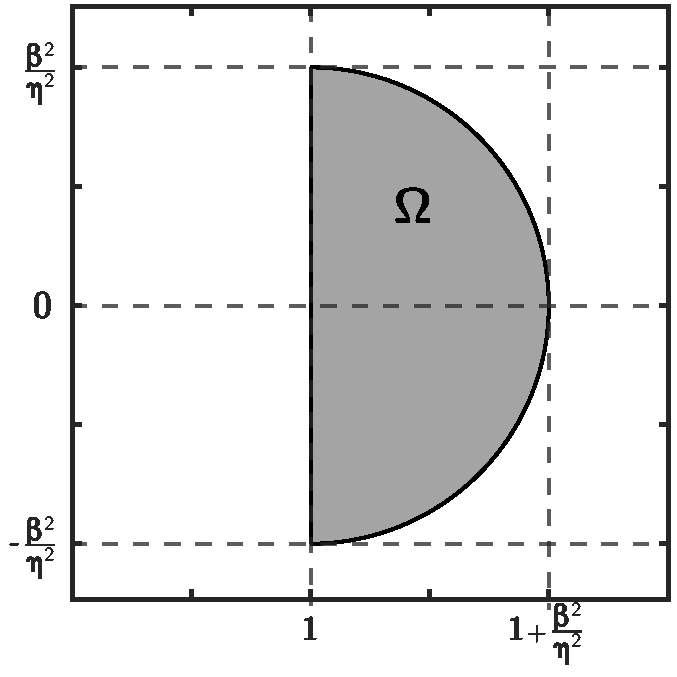
\includegraphics[width = 0.3\textwidth]{fov.pdf}
\caption{}
\label{fig:bound}
\end{figure}
\end{theorem}
%

%
\begin{corollary}\label{cor:gmres}
Let $\pi_k$ denote the set of consistent polynomials of degree $k$. Then the ideal GMRES bound
(an upper bound in operator norm on worst-case convergence) on convergence after $k$ iterations
applied to the preconditioned operator $\mathcal{P}_A$ \eqref{eq:prec1} is bounded by
\begin{align*}
\min_{p\in\pi_k} \|p(\mathcal{P}_A)\| \leq 2\left(\frac{\beta^2/\eta^2}{2 + \beta^2/\eta^2}\right)^k.
\end{align*}
\end{corollary}
\begin{proof}
For operator $M$, let $\nu(M)$ denote the distance of $W(M)$ from the origin. In \todo{cite Liesen},
they define $\cos(\beta) := \nu(M) / r(M)$, and prove that worst-case convergence of GMRES applied
to operator $M$ is bounded by (see Lemma 3.2)
%
\begin{align}\label{eq:gmres}
\min_{p\in\pi_k} \|p(M)\| \leq 2\left(\frac{1-\cos\beta}{1+\cos\beta}\right)^k.
\end{align}
%
For $M = \mathcal{P}_A$, we have $\nu(\mathcal{P}_A)= 1$ and $r(\mathcal{P}_A) \leq 1+\beta^2/\eta^2$.
Plugging into \eqref{eq:gmres} completes the proof. 
\end{proof}
%

{\color{blue}
\begin{itemize}
	\item Comment on size of $\eta$ and $\beta$ and convergence bounds for GMRES. Largest (squared)
	ratio I have seen is $\sim 4.29$ for RadauIIA(11), but another eigenvalue pair for the same
	scheme had ratio $\sim 0.04$, so the seem to even out.

	\item Is $\eta > 0$ always? Looks like it for everything I have tested, would be nice to
	say something general.. If not, need to confirm it holds for lots of standard methods.
	This is important assumption in above analysis.

	\item Classical GMRES convergence results based on $\lambda_{\textnormal{min}}((\mathcal{P}_A+
	\mathcal{P}_A^T)/2)$ and $\lambda_{\textnormal{max}}(\mathcal{P}_A^T\mathcal{P}_A)$ can also
	be applied, yielding a less tight result of $\left(\frac{\beta^2/\eta^2}{1 + \beta^2/\eta^2}\right)^{k/2}$.
	The field-of-values is $2-4\times$ tighter, and deriving the field-of-values also reflects the
	nice conditioning of the operator. 

\end{itemize}
}

% ----------------------------------------------------------------------------------------------------------- %
% ----------------------------------------------------------------------------------------------------------- %
\subsection{Preconditioning quadratic polynomials}

In practice, we generally do not want to directly form preconditioners for a quadratic
polynomial in $\mathcal{L}$, not the least because even forming such an operator is 
expensive in parallel. Instead, the previous section suggests we can use two successive 
applications of a preconditioner for $(\alpha I - \mathcal{L})$. If $(\alpha I - \mathcal{L})^{-1}$
is applied twice to the \textit{action} of $(\alpha^2+\beta^2)I - 2\alpha\mathcal{L} + \mathcal{L}^2$,
\Cref{th:fov} proves that the preconditioned operator is very well conditioned and GMRES
will converge rapidly (see also \Cref{cor:gmres}). However, in practice, fully converging
$(\alpha I - \mathcal{L})^{-1}$ is not desirable --  even if GMRES converges rapidly,
if each iteration requires a full linear solve, the resulting method remains moderately
expensive. 
Here, we propose applying GMRES to $(\alpha^2+\beta^2)I - 2\alpha\mathcal{L} + \mathcal{L}^2$
by computing the operator's action (that is, not fully constructing it), and preconditioning
each GMRES iterations with \textit{two} applications of a sparse parallel preconditioner for
$(\alpha I - \mathcal{L})$, representing the action of $(\alpha I - \mathcal{L})^{-2}$. 



{\color{blue}
\begin{itemize}
	\item I am thinking each GMRES iteration we only do a few (or even one?) AMG iterations
	for each application of $(\alpha I - \mathcal{L})$, hoping that at the end it doesn't
	really take more iterations than if we were to directly apply AMG preconditioned GMRES
	to $(\alpha I - \mathcal{L})^2$.

	\item We are actually preconditioning a much worse-conditioned operator. The $+\beta^2$
	term we get in the operator (rather than preconditioner) shifts the field-of-values 
	positive and away from the origin by $\beta$. Hopefully this pans out by observing
	rapid convergence..

	\item One thing I am really puzzled by -- by formulating based on $A_0^{-1}$, the
	eigenvalues in my tests appear to be fairly large in magnitude. E.g., eigenvalues of
	$A_0$ are $\sim 0.1$ and eigenvalues of $A_0^{-1}$ are $\sim 5$. If this is true and we
	can get away with solving $(\eta I -\mathcal{L})$ for $\eta \sim 10\times$ larger than
	eigenvalues of $A_0$, that could be huge. In theory such systems would likely be way
	better conditioned. It also seems too good to be true/not very intuitive to solve a
	system with such a big shift when our actual time step is $\ll$..

\end{itemize}
}


% ----------------------------------------------------------------------------------------------------------- %
% ----------------------------------------------------------------------------------------------------------- %
% ----------------------------------------------------------------------------------------------------------- %
\newpage
\section{The time-dependent case}


{\color{blue}

\begin{itemize}
\item What happens when $\mathcal{L}$ is time-dependent? For the $2\times 2$ case, it is
likely that $\alpha_{12}\alpha_{21}$ is positive, in which case we can use a similar
motivation as above to to precondition $P_{\mathcal{L}}$ with $(\alpha_{11}I - \mathcal{L}_1)^{-1}
(\alpha_{22}I - \mathcal{L}_2)^{-1}$. How would this extend to 3/4 stages though?
For fixed-time, this is not as desirable because have to solve two different
matrices, whereas to address conjugate case above we solve both with $\alpha$.

\item We can do maybe handle time dependence formally -- there is theory on matrices over
non-commutative rings. There is even a closed form for the inverse based on quasi-determinants,
where we can express each element of $A^{-1}$ (https://en.wikipedia.org/wiki/Quasideterminant).

\item The original form before we factor out $A_0\otimes I$ is almost a Manin matrix. A Manin
matrix is a specific kind of matrix over a noncommutative ring where traditional linear
algebra results hold. Could use Manin inverse as a preconditioner? Can we scale $A_0$
in any way such that it is a Manin matrix? Looking at $2\times 2$, this doesn't look
promising.


\end{itemize}

}

% ----------------------------------------------------------------------------------------------------------- %
% ----------------------------------------------------------------------------------------------------------- %
\subsection{Two stages}

Consider the case of two fully implicit stages. Then we need to invert a block linear system
$\mathcal{M}_2\mathbf{s} = \mathbf{r}$, given by
%
\begin{align}\label{eq:Mnt}
\begin{bmatrix} \alpha_{11} I - \mathcal{L}_1 & \alpha_{12}I \\ \alpha_{21}I & \alpha_{22}I - \mathcal{L}_2\end{bmatrix}
	\begin{bmatrix}\mathbf{s}_1 \\ \mathbf{s}_2 \end{bmatrix} = 
	\begin{bmatrix}\mathbf{r}_1 \\ \mathbf{r}_2 \end{bmatrix}.
\end{align}
%
In the context of $2\times 2$ block operators, the key to inverting the matrix is inverting one of
the Schur complements. Define the matrix polynomials
%
\begin{align*}
P_{\mathcal{L}} := (\alpha_{11}I - \mathcal{L}_1)(\alpha_{22}I - \mathcal{L}_2) - \alpha_{12}\alpha_{21}I, \\
Q_{\mathcal{L}} := (\alpha_{22}I - \mathcal{L}_2)(\alpha_{11}I - \mathcal{L}_1) - \alpha_{12}\alpha_{21}I,
\end{align*}
%
and consider both Schur complements,
%
\begin{align*}
S_{22} & = \alpha_{22} I - \mathcal{L}_2 - \alpha_{12}\alpha_{21}(\alpha_{11} I - \mathcal{L} )^{-1} \\
& = \left[ ( \alpha_{22} I - \mathcal{L}_2)(\alpha_{11} I - \mathcal{L}_1) - \alpha_{12}\alpha_{21}I \right]
	(\alpha_{11} I - \mathcal{L}_1 )^{-1} \\
& = Q_{\mathcal{L}}(\alpha_{11} I - \mathcal{L}_1 )^{-1} \\
& = (\alpha_{11} I - \mathcal{L}_1 )^{-1}P_{\mathcal{L}} \\
S_{11} & = P_{\mathcal{L}}(\alpha_{22} I - \mathcal{L}_2 )^{-1} \\
& = (\alpha_{22} I - \mathcal{L}_2 )^{-1}Q_{\mathcal{L}}.
\end{align*}
%
%Note that 
%%
%\begin{align*}
%P_{\mathcal{L}} & = (\alpha_{22} I + \mathcal{L}_2 )Q_{\mathcal{L}}(\alpha_{22} I + \mathcal{L}_2 )^{-1} \\
%& = (\alpha_{11} I + \mathcal{L}_1 )^{-1} Q_{\mathcal{L}}(\alpha_{11} I + \mathcal{L}_1 ).
%\end{align*}
%%
Appealing to the closed form inverse of $2\times 2$ block matrices derived from a block LDU decomposition,
we can then write $\mathcal{M}_2^{-1}$ in terms of the Schur complements:
%
\begin{align}
\begin{bmatrix} \alpha_{11} I - \mathcal{L}_1 & \alpha_{12}I \\ \alpha_{21}I & \alpha_{22}I - \mathcal{L}_2\end{bmatrix} ^{-1}
	& = \begin{bmatrix}  (\alpha_{22} I - \mathcal{L}_2 )P_{\mathcal{L}}^{-1} & -\alpha_{12}Q_{\mathcal{L}}^{-1} \\
		-\alpha_{21}P_{\mathcal{L}}^{-1} & (\alpha_{11} I - \mathcal{L}_1 )Q_{\mathcal{L}}^{-1} \end{bmatrix} \nonumber\\
& = \begin{bmatrix} \alpha_{22} I - \mathcal{L}_2  & -\alpha_{12}I \\ -\alpha_{21}I & \alpha_{11} I - \mathcal{L}_1 \end{bmatrix} 
	\begin{bmatrix} P_{\mathcal{L}}^{-1}  & \mathbf{0} \\ \mathbf{0} & Q_{\mathcal{L}}^{-1} \end{bmatrix}.\label{eq:Minv}
\end{align}
%
\tcb{Note, this more or less exactly takes the form of a scalar $2\times 2$ matrix inverse, replacing
the $1/det$ with the right scaling by the polynomial inverses.. We can also restructure to pull
polynomials out of the left }


% ----------------------------------------------------------------------------------------------------------- %
\subsubsection{Two stages}

Returning to the case of two stages, by assuming $\mathcal{L}_1 = \mathcal{L}_2$ we have
$P_{\mathcal{L}} = Q_{\mathcal{L}} := P_2(\mathcal{L})$. Then, $\mathcal{M}_2^{-1}$ \eqref{eq:Minv} can
be applied through two applications of $P_2(\mathcal{L})^{-1}$, along with some additional mat-vecs and
vector addition. Note that $P_2(\mathcal{L})$ is a quadratic polynomial in $\mathcal{L}$, which can be
solved in two steps by factoring \eqref{eq:fac} and applying the successive inverses
$(\lambda_1 I - \mathcal{L})^{-1}(\lambda_2 I - \mathcal{L})^{-1}$, where $\lambda_1,\lambda_2$ are
the eigenvalues of $\boldsymbol{\alpha} = A_0^{-1}$. Note, in the $2\times 2$ case these have a
relatively simple algebraic structure, 
%
\begin{align*}
\lambda_1,\lambda_2 & = \frac{1}{2} \left( \alpha_{11} + \alpha_{22} \pm \sqrt{ (\alpha_{11} + \alpha_{22})^2 - 4 ( \alpha_{11}\alpha_{22} - \alpha_{12}\alpha_{21})} \right).
\end{align*}
%



% ----------------------------------------------------------------------------------------------------------- %
\subsubsection{Three stages}

For nonsingular scalar $3\times 3$ matrix $A$, the inverse is given by 
%
\begin{align}
{A}^{-1} =
\begin{bmatrix}
	a_{11} & a_{12} & a_{13}\\ a_{21} & a_{22} & a_{23} \\ a_{31} & a_{32} & a_{33}\\
\end{bmatrix}^{-1} =
\det({A})^{-1} \begin{bmatrix}
	\, A_{11} & \, A_{12} & \,A_{13} \\ \, A_{21} & \, A_{22} & \,A_{23} \\ \, A_{31} & \,A_{32} & \, A_{33}\\
\end{bmatrix},\label{eq:3inv}
\end{align}
%
with elements defined by
%
\begin{alignat*}{6}
A_{11} &={}&  (a_{22}a_{33} - a_{23}a_{32}), &\quad&
    A_{12} &={}& -(a_{12}a_{33} - a_{13}a_{32}), &\quad&
    A_{13} &={}&  (a_{12}a_{23} - a_{13}a_{22}), \\
A_{21} &={}& -(a_{21}a_{33} - a_{23}a_{31}), &\quad&
    A_{22} &={}&  (a_{11}a_{33} - a_{13}a_{31}), &\quad&
    A_{23} &={}& -(a_{11}a_{23} - a_{13}a_{21}), \\
A_{31} &={}&  (a_{21}a_{32} - a_{22}a_{31}), &\quad&
    A_{32} &={}& -(a_{11}a_{32} - a_{12}a_{31}), &\quad&
    A_{33} &={}&  (a_{11}a_{22} - a_{12}a_{21}),
\end{alignat*}
%
and determinant $\det({A}) = a_{11}A_{11}+a_{12}A_{21}+a_{13}A_{31}$.

In our case, consider 
%
\begin{align}\label{eq:Mnt}
\mathcal{M}_3 &:= \begin{bmatrix} (\alpha_{11} I + \mathcal{L}) & \alpha_{12}I & \alpha_{13}I \\
    \alpha_{21}I & (\alpha_{22}I + \mathcal{L}) & \alpha_{23} I \\
    \alpha_{31}I & \alpha_{32}I & (\alpha_{33} I + \mathcal{L}) \end{bmatrix}.
\end{align}
%
Define $\mathcal{N}_3$ as a block $3\times 3$ matrix with entries of $A^{-1}$ as in \eqref{eq:3inv},
excluding the determinant. Plugging in, we have entries of $\mathcal{N}_3$ given by
%
\begin{align*}
A_{11} &=  (\alpha_{22}I - \mathcal{L})(\alpha_{33} I - \mathcal{L}) - \alpha_{23}\alpha_{32}I, \\
    A_{12} &= -\alpha_{12}(\alpha_{33} I - \mathcal{L}) + \alpha_{13}\alpha_{32}I, \\
    A_{13} &=  \alpha_{12}\alpha_{23} I - \alpha_{13}(\alpha_{22}I - \mathcal{L}), \\
A_{21} &= -\alpha_{21}(\alpha_{33} I - \mathcal{L}) + \alpha_{23} \alpha_{31}I, \\
    A_{22} &=  (\alpha_{11} I - \mathcal{L})(\alpha_{33} I - \mathcal{L}) - \alpha_{13}\alpha_{31}I, \\
    A_{23} &= -\alpha_{23}(\alpha_{11} I - \mathcal{L}) + \alpha_{13}\alpha_{21}I, \\
A_{31} &=  \alpha_{21}\alpha_{32}I - \alpha_{31}(\alpha_{22}I - \mathcal{L}), \\
    A_{32} &= -\alpha_{32}(\alpha_{11} I - \mathcal{L}) + \alpha_{12}\alpha_{31}I, \\
    A_{33} &=  (\alpha_{11} I - \mathcal{L})(\alpha_{22}I - \mathcal{L}) - \alpha_{12}\alpha_{21}I.
\end{align*}
%
Working through the details, it is striaghtforward to confirm that $\mathcal{N}_3\mathcal{M}_3$
is a block-diagonal matrix, with diagonal blocks given by the (block) determinant of $\mathcal{M}_3$,
%
\begin{align*}
D & = (\alpha_{11}I - \mathcal{L}) (\alpha_{22}I - \mathcal{L})(\alpha_{33} I - \mathcal{L}) -
	\alpha_{23}\alpha_{32}(\alpha_{11}I - \mathcal{L}) - \\
& \hspace{5ex} 
	\alpha_{13}\alpha_{31}(\alpha_{22}I - \mathcal{L}) -
	\alpha_{12}\alpha_{21}(\alpha_{33}I - \mathcal{L}) + (\alpha_{13}\alpha_{32}\alpha_{21} + \alpha_{12}\alpha_{23}\alpha_{31})I.
\end{align*}
%
Similar to the $2\times 2$ case (albeit algebraically more complicated), this is a cubic polynomial in
$\mathcal{L}$. By computing the roots of this polynomial, we can construct error propagation of a
three-stage fixed-point iteration that produces the exact inverse of $\mathcal{D}$. 


%
{\color{blue}A few more thoughts:
\begin{itemize}
\item Working through the algebra, the cancellation does not fully happen if $\mathcal{L}_i$
is time-dependent. However, a lot of it does. There will be some off-diagonal terms that take
the form, for example,
%
\begin{align*}
(\alpha_{11}I - \mathcal{L}_1)(\alpha_{22}I - \mathcal{L}_2) - 
	(\alpha_{22}I - \mathcal{L}_2)(\alpha_{11}I - \mathcal{L}_1)
& = \mathcal{L}_1\mathcal{L}_2 - \mathcal{L}_2\mathcal{L}_1.
\end{align*}
%
This provides a nice theoretical tool to analyze what is going on. It is possible these are often
quite small. Moreover, we may be able to choose an ordering where these terms only occur on,
say, the stritly lower triangular part, in which case a block-triangular preconditioning would also
be exact. 

\end{itemize}
}
%

% ----------------------------------------------------------------------------------------------------------- %
% ----------------------------------------------------------------------------------------------------------- %
% ----------------------------------------------------------------------------------------------------------- %
\section{Parallel in time}

\begin{itemize}
	\item For pAIR or MGRiT, can we do a $p$-multigrid approach, where we solve order $p$ MGRIT
	via a set of $p$ MGRiT/pAIR solves for order 1? 
	\item Another (simpler) possibility is use global Krylov only applied to the solution vector,
	and precondition a high-order time integrator with pAIR built on a low-order time integrator.
	This could also be done as a two-grid method, where we do high-order stage integration as a
	relaxation coupled with a pAIR solve with a low-order time integrator. This could couple well
	if I come up with a good way to do fully implicit IRK solves, we could use that on the finest
	grid. Or, we could just use full implicit IRK as the operator, relax w/ high order SDIRK,
	then coarse-grid correct with pAIR on low-order SDIRK (is this SDC or PFAST?)
\end{itemize}


% ----------------------------------------------------------------------------------------------------------- %
% ----------------------------------------------------------------------------------------------------------- %
\subsection{Precondition HO with LO}


Let $\Phi$ denote a single step of our high-order (fine-grid) Runge-Kutta operator and
$\Psi$ a single step of our low-order (coarse-grid) operator. Then error propagation for
preconditioning a global time-stepping scheme base don $\Phi$ with a low-order scheme 
based on $\Psi$ is given by 
%
\begin{align*}
I - B_\Delta^{-1} A & =
	{\begin{bmatrix} \mathbf{0} \\ I & \mathbf{0} \\ \Psi & I & \mathbf{0} \\ \vdots & \vdots & \ddots & \ddots \\ \Psi^{N_c-2} & \Psi^{N_c-3} & ... & I  & \mathbf{0} \end{bmatrix} } \textnormal{{diag}}{(\Psi - \Phi)}.
\end{align*}
%
Here we have assumed $\Phi$ and $\Psi$ to be linear and independent of time, but that
is not necessary. The (linearized) time-dependent setting has the same form as above,
but with products of $\Psi$ evaluated at successive (discrete) times.

Note this is analogous to two-level convergence of MGRiT. Necessary and sufficient conditions
for convergence are given by the temporal approximation property,
%
\begin{definition}[Temporal approximation property]
Let $\Phi$ denote a fine-grid time-stepping operator and $\Psi$ denote a coarse-grid time-stepping operator, for all time points,
with coarsening factor $k$. Then, $\Phi$ satisfies an F-relaxation temporal approximation property with power $p$
(F-TAP$_p$), with respect to $\Psi$, with constant $\varphi_{F,p}$, if, for all vectors $\mathbf{v}$,
\begin{align}\label{eq:tap_f}
\|(\Psi - \Phi^k)^p\mathbf{v}\| \leq \varphi_{F,p} \left[\min_{x\in[0,2\pi]} \left\| (I - e^{\mathrm{i}x}\Psi )^p\mathbf{v}\right\| \right].
\end{align}
Similarly, $\Phi$ satisfies an FCF-relaxation temporal approximation property with power $p$ (FCF-TAP$_p$), with
respect to $\Psi$, with constant $\varphi_{FCF,p}$, if, for all vectors $\mathbf{v}$,
\begin{align}\label{eq:tap_fcf}
\|(\Psi - \Phi^k)^p\mathbf{v}\| \leq \varphi_{FCF,p}\left[\min_{x\in[0,2\pi]} \left\| (\Phi^{-k}(I - e^{\mathrm{i}x}\Psi) )^p\mathbf{v}\right\| \right].
\end{align}
\end{definition}
%
For the F-relaxation case, we have $k = 1$. The analogous FCF context here would presumably
correspond to doing a complete fine-grid solve on processor. The downside is this is kind of
expensive. However, if we treat $\Phi$ as an explicit scheme, with the stages and implicit 
solves included, just the action of the operator will be expensive to compute. I think it will
be important to somehow consider the RK scheme expanded, so that when we apply a coarse-grid
preconditioner, computing the action of the operator can be done explicitly and doesn't require
computing a bunch of inverses...

L-stability appears to be important here, and is not perfect. But, with just F-relaxation, then
we don't even need to solve the fine grid implicit discretization. Need to check how this could
work with fully implicit fine grid discretization, preconditioned with BE.. Would be cool if that
could be effective. 


% ----------------------------------------------------------------------------------------------------------- %
% ----------------------------------------------------------------------------------------------------------- %
\subsection{A multigrid or block preconditioning perspective}

Let $A$ and $\mathbf{b}$ correspond to Butcher tableaux,
%
\begin{align*}
\hspace{-6ex}\implies \hspace{3ex}\mathbf{u}_{i+1} & = \mathbf{u}_i + \delta t\sum_{i=1}^{s} b_i\mathbf{k}_i,
\end{align*}
%
and let $\hat{\mathbf{u}} = [\mathbf{u}_0, \mathbf{u}_1,...]$ denote the space-time solution
at times $t_0,t_1,...$. Then the full space-time linear system takes the form $A\hat{\mathbf{u}}
= \hat{\mathbf{g}}$, where
%
\begin{align*}
\hspace{-4ex}A = 
\begin{blockarray}{c c c c c c} \textnormal{\underline{\tiny{$t_0$}}} & \textnormal{\tiny(stages)} &
	\textnormal{\underline{\tiny{$t_1$}}} &  \textnormal{\tiny(stages)} & \textnormal{\underline{\tiny{$t_2$}}} & ... \\
\begin{block}{(c c c c c c)}
	I &  \\
	-\delta t(\mathbf{1}_n \otimes \mathcal{L}) & I - \delta t A\otimes \mathcal{L} &\\
	-I & -\mathbf{b}\otimes I & I \\ 
	& & -\delta t(\mathbf{1}_n \otimes \mathcal{L}) & I - \delta t A\otimes \mathcal{L} &  \\
	& & -I & -\mathbf{b}\otimes I & I \\
	&&& \ddots\text{\hspace{4ex}}  & \ddots\text{\hspace{8ex}}  & \ddots \\
	\end{block}
\end{blockarray}\hspace{1ex}.
\end{align*}
%
Note, for ease of notation here, we have assumed that $\mathcal{L}$ is independent of time
and the stage matrix can be written as a Kronecker product. However, for time-dependent
problems, the space-time matrix takes a similar structure, but the stage-matrix must be
written explicitly as a block $s\times s$ matrix. 
Now, let us denote all intermediate RK stages as F-points and time-points as C-points. 
Eliminating the F-points in a Schur complement sense yields the reduced MGRiT-style
system,
%
\begin{align*}
A & = \begin{blockarray}{c c c c c} \textnormal{\underline{\tiny{$t_0$}}} & \textnormal{\underline{\tiny{$t_1$}}} & ... &... &\textnormal{\underline{\tiny{$t_N$}}} \\
	\begin{block}{(c c c c c)}
	I & & & & \\
	-\Phi & I & & &\\
	 & -\Phi& I & & \\
	 &  & \ddots & \ddots  & \\
	 &  & & -\Phi & I \\
	\end{block}
	\end{blockarray} \hspace{1ex}, 
\end{align*}
%
where
%
\begin{align}\label{eq:mgrit}
\Phi & = I + \delta t\mathbf{b}_0^T\otimes I \left(I - \delta t A_0\otimes \mathcal{L}\right)^{-1} (\mathbf{1}_n \otimes \mathcal{L}).
\end{align}
%
As previously, this takes a more complicated but similar form if $\mathcal{L}$ is
time-dependent.\\
\\
I see two nice ways to think about this:
%
\begin{enumerate}
	\item The simplest is a block-preconditioning approach. Reordering the matrix by stages
	and then time-points, We will use a block lower-triangular preconditioner. If we exactly
	invert the F-block (solve all RK stages exactly) followed by inverting the Schur complement,
	we converge in two iterations. Of course in this case, that is just sequential time stepping.
	But, we could approximate our Schur complement with a space-time solve using a low-order 
	integrator (BE?) and couple this with an F-relaxation (some inexact solution to the
	stage matrices). Note, theory and practice have generally indicated that if one solve is
	not exact, the other also does not need to be, so we probably shouldn't solve the stages
	exactly. This makes me think we might be able to let the true RK scheme be a high-order
	fully implicit RK scheme, and precondition this with an SDIRK scheme on stage integration.

	\item Above can also be thought of in some sense as a non-Galerkin multigrid method.
	But, we developed a decent two-grid theoretical framework for AIR. I wonder if we can
	construct $R$ and $P$ so that approximating high-order $\Phi$ on the coarse-grid with
	backward Euler is actually a Petrov-Galerkin multigrid method, that is, $RAP$ directly
	leads to a matrix analogous to \eqref{eq:mgrit} but with $\Phi\sim$ backward Euler
	(or some other one-stage method)?

\end{enumerate}





\end{document}